\documentclass[a4paper,twoside]{article}
\usepackage[T1]{fontenc}
\usepackage[bahasa]{babel}
\usepackage{graphicx}
\usepackage{graphics}
\usepackage{float}
\usepackage[cm]{fullpage}
\pagestyle{myheadings}
\usepackage{etoolbox}
\usepackage{setspace} 
\usepackage{lipsum} 
\setlength{\headsep}{30pt}
\usepackage[inner=2cm,outer=2.5cm,top=2.5cm,bottom=2cm]{geometry} %margin
% \pagestyle{empty}

\makeatletter
\renewcommand{\@maketitle} {\begin{center} {\LARGE \textbf{ \textsc{\@title}} \par} \bigskip {\large \textbf{\textsc{\@author}} }\end{center} }
\renewcommand{\thispagestyle}[1]{}
\markright{\textbf{\textsc{Laporan Perkembangan Pengerjaan Skripsi\textemdash Sem. Genap 2019/2020}}}

\onehalfspacing
 
\begin{document}

\title{\@judultopik}
\author{\nama \textendash \@npm} 

%ISILAH DATA BERIKUT INI:
\newcommand{\nama}{Muhammad Dipo Putra Wandara}
\newcommand{\@npm}{2016730091}
\newcommand{\tanggal}{22/11/2019} %Tanggal pembuatan dokumen
\newcommand{\@judultopik}{Pengujian Berbasis \textit{Behavior Specification}} % Judul/topik anda
\newcommand{\kodetopik}{RCP4702}
\newcommand{\jumpemb}{1} % Jumlah pembimbing, 1 atau 2
\newcommand{\pembA}{Raymond Chandra Putra}
\newcommand{\pembB}{-}
\newcommand{\semesterPertama}{47 - Genap 19/20} % semester pertama kali topik diambil, angka 1 dimulai dari sem Ganjil 96/97
\newcommand{\lamaSkripsi}{2} % Jumlah semester untuk mengerjakan skripsi s.d. dokumen ini dibuat
\newcommand{\kulPertama}{Skripsi 1} % Kuliah dimana topik ini diambil pertama kali
\newcommand{\tipePR}{C} % tipe progress report :
% A : dokumen pendukung untuk pengambilan ke-2 di Skripsi 1
% B : dokumen untuk reviewer pada presentasi dan review Skripsi 1
% C : dokumen pendukung untuk pengambilan ke-2 di Skripsi 2

% Dokumen hasil template ini harus dicetak bolak-balik !!!!

\maketitle

\pagenumbering{arabic}

\section{Data Skripsi} %TIDAK PERLU MENGUBAH BAGIAN INI !!!
Pembimbing utama/tunggal: {\bf \pembA}\\
Pembimbing pendamping: {\bf \pembB}\\
Kode Topik : {\bf \kodetopik}\\
Topik ini sudah dikerjakan selama : {\bf \lamaSkripsi} semester\\
Pengambilan pertama kali topik ini pada : Semester {\bf \semesterPertama} \\
Pengambilan pertama kali topik ini di kuliah : {\bf \kulPertama} \\
Tipe Laporan : {\bf \tipePR} -
\ifdefstring{\tipePR}{A}{
			Dokumen pendukung untuk {\BF pengambilan ke-2 di Skripsi 1} }
		{
		\ifdefstring{\tipePR}{B} {
				Dokumen untuk reviewer pada presentasi dan {\bf review Skripsi 1}}
			{	Dokumen pendukung untuk {\bf pengambilan ke-2 di Skripsi 2}}
		}
		
\section{Latar Belakang}
Pengujian perangkat lunak merupakan salah satu tahapan dari \textit{software development life cycle}. \textit{Software Development Life Cycle}(SDLC) merupakan metodologi dari pengembangan perangkat lunak, metode ini dibagi menjadi beberapa fase seperti\textit{ analysis, design,  coding,  testing, installation} dan \textit{maintenance}. Pengujian perangkat lunak adalah proses untuk mencari kesalahan pada setiap komponen perangkat lunak, mencatat hasilnya, mengevaluasi setiap aspek pada setiap komponen dan mengevaluasi fitur-fitur dari perangkat lunak yang akan dikembangkan. Pengujian pada perangkat lunak merupakan tahapan yang wajib dilakukan sebelum perangkat lunak tersebut digunakan, agar memastikan sudah tidak ada kesalahan/\textit{bug} pada perangkat lunak yang sedang dikembangkan. Pengujian perangkat lunak memakan sumberdaya yang berat, baik itu waktu maupun waktu maupun tenaga kerja, karena untuk melakukan pengujian perangkat lunak dibutuhkan pengembang dengan keahlian \textit{Software Quality Assurance}(SQA). SQA yang bertanggung jawab untuk memastikan bahwa perangkat lunak yang sedang dikembangkan bebas dari \textit{bug} agar siap untuk dirilis dan digunakan oleh pengguna.

Pengujian perangkat lunak memiliki beberapa tahapan, yaitu:
\begin{itemize}
	\item \textit{Unit Test} : Tes komponen secara individu.
	\item \textit{Integration Test} : Tes komponen yang sudah terintegrasi.
	\item \textit{System Test} : Tes keseluruhan sistem.
	\item \textit{Acceptance Test} : Tes sistem akhir.
\end{itemize}
Kita akan membahas tentang \textit{unit testing}, \textit{unit testing} merupakan tahapan pertama dari pengujian perangkat lunak. \textit{Unit Testing} adalah proses pengujian bagian kode secara individu, suatu komponen, untuk menentukan apakah kode tersebut berfungsi dengan semestinya. Salah satu teknik untuk membuat \textit{unit testing} yaitu dengan code generation. \textit{Code generation} adalah teknik membuat suatu program yang membuat program lain. Menggunakan \textit{code generation} untuk \textit{unit testing} membuatnya dapat digunakan dalam jangka yang panjang.

Salah satu teknik pengembangan perangkat lunak ialah \textit{Test-Driven Development}(TDD). Test-Driven Development (TDD) adalah praktik pengembangan yang menggunakan \textit{unit test} untuk menentukan, merancang, dan memverifikasi kode yang akan ditulis. Sebelum menerapkan fungsionalitas, pengembang menulis \textit{unit test} yang sengaja digagalkan untuk menunjukkan bagaimana fungsi ini seharusnya bekerja. Pada saat yang sama, pengujian gagal ini juga membuktikan bahwa implementasi saat ini belum mendukung fungsionalitas yang baru. Baru setelah itu pengembang menulis kode program. Setelah \textit{unit testing} berlalu, pengembang tahu bahwa fungsionalitas telah berhasil diimplementasikan. Pada tahap ini, mereka dapat meninjau kode mereka untuk merapikan dan menyempurnakan desain. Ada satu lagi teknik pengembangan perangkat lunak, yang dianggap para ahli memiliki kelebihan yang TDD tidak miliki, yaitu \textit{Behaviour-Driven Development}(BDD).

\textit{Behaviour-Driven Development}(BDD) merupakan pengembangan dari TDD untuk menyelesaikan masalah yang ada pada TDD. BDD adalah seperangkat praktik rekayasa perangkat lunak yang dirancang untuk membantu tim membangun dan memberikan perangkat lunak yang memfasilitasi komunikasi antara anggota tim proyek dan pemangku kepentingan bisnis.

Prinsip inti dari BDD adalah "orang bisnis dan teknologi harus merujuk ke sistem yang sama dengan cara yang sama". Berbeda dengan TDD yang berpatokan pada tes untuk pengembang lebih jauh program yang akan digunakan, BDD berpatokan pada keinginan \textit{stakeholder} untuk mengembangkan programnya. Untuk mencapai kesepakatan antara pengembang dan \textit{stakeholder}, maka dibutuhkan \textit{language} untuk menspesifikasikan \textit{behaviour} sebuah sistem agar kedua pihak paham, dan dapat mewujudkan hal berikut:
\begin{itemize}
\item \textit{Stakeholder} untuk menentukan persyaratan dari perspektif bisnis.
\item Analis bisnis untuk melampirkan contoh konkret (skenario atau \textit{acceptance tests}) yang menjelaskan \textit{behaviour} sistem.
\item Pengembang untuk mengimplementasikan \textit{behaviour} sistem yang diperlukan secara TDD.
\end{itemize}
	
Pengujian dengan basis \textit{behaviour specification} akan berfokus kepada hal yang \textit{stakeholder} harapkan pada suatu sistem dengan \textit{behaviour} yang sudah di spesifikasikan. Pengujian akan berawal dengan membuat \textit{scenario} yang berisi:
\begin{enumerate}
\item \textit{Context/Starting state} : Posisi awal sistem sebelum terjadinya suatu \textit{event}.
\item \textit{Event} : \textit{Task} yang dilakukan oleh pengguna pada sistem.
\item \textit{Outcome} : Hasil yang diharapkan dari sistem.
\end{enumerate}
Pengembang akan menjadikan \textit{scenario} sebagai patokan dasar bekerjanya suatu sistem, dan akan melakukan pengujian berbasis \textit{scenario}. Pengujian dilakukan untuk memastikan bahwa sistem sudah bekerja sesuai apa yang \textit{stakeholder} harapkan, dan jika \textit{scenario} berhasil dilakukan, maka sistem sudah siap untuk digunakan.

Pada skripsi ini akan dibangun sebuah perangkat pengujian yang mengimplementasi \textit{behaviour specification} untuk menguji sebuah perangkat lunak.
\section{Rumusan Masalah}
\begin{itemize}
\item Bagaimana cara kerja pengujian berbasis \textit{behavior specification}?
\item Bagaimana implementasi perangkat lunak yang dapat menguji program berbasis \textit{behavior specification} ?	
\end{itemize}
\section{Tujuan}
\begin{itemize}
\item Mempelajari cara kerja pengujian berbasis \textit{behaviour specification}
\item Menghasilkan perangkat penguji yang dapat menguji sebuah perangkat lunak berbasiskan \textit{behaviour specification}.
\end{itemize}
\section{Detail Perkembangan Pengerjaan Skripsi}
Detail bagian pekerjaan skripsi sesuai dengan rencana kerja/laporan perkembangan terakhir :
	\begin{enumerate}
		\item \textbf{Studi literatur mengenai pengujian perangkat lunak, \textit{unit testing}, dan \textit{behaviour specification}}\\
		{\bf Status :} Ada sejak rencana kerja skripsi.\\
		{\bf Hasil :} Studi literatur telah dilakukan dengan membaca berbagai buku yang berkaitan dengan pengujian perangkat, \textit{unit testing}, dan \textit{behaviour specification}. Buku yang digunakan untuk referensi yaitu \textit{Software Testing: A Craftsman’s Approach, Fourth Edition}, \textit{Software Testing and Continuous Quality Improvement, Third Edition}, \textit{Testing Python: Applying Unit Testing, TDD, BDD and Acceptance Testing}, \textit{BDD in Action: Behavior-Driven Development for the whole software lifecycle}, Software Testing and Quality Assurance Theory and Practice, dan The Journal of Systems \& Software.
	
\section*{Pengujian Perangkat Lunak}	
Pandangan umum pengujian perangkat lunak adalah bahwa kegiatan ini adalah untuk menemukan \textit{bug}. Tujuan pengujian perangkat lunak adalah untuk memenuhi syarat kualitas program perangkat lunak dengan mengukur atribut dan kemampuannya terhadap ekspektasi dan standar yang berlaku. Pengujian perangkat lunak juga menyediakan informasi berharga untuk upaya pengembangan perangkat lunak.

Semua orang ingin perangkat lunak yang memiliki kualitas tinggi. Manajer tahu bahwa mereka menginginkan kualitas tinggi, pengembangan perangkat lunak tahu mereka ingin menghasilkan produk yang berkualitas, dan pengguna bersikeras bahwa perangkat lunak bekerja secara konsisten dan dapat diandalkan.

Banyak kelompok kualitas perangkat lunak mengembangkan \textit{software quality assurance plan}, dimana hal itu sama dengan \textit{test plans}. Rencana jaminan kualitas perangkat lunak dapat mencakup berbagai kegiatan di luar yang termasuk dalam rencana tes. \textit{Quality assurance plan} mencakup keseluruhan kualitas, rencana pengujian adalah salah satu alat kontrol kualitas dari rencana jaminan kualitas.

Pada pembahasan pengujian perangkat lunak, ada \textit{term} yang biasa digunakan, yaitu:
\begin{itemize}
\item \textbf{Error} --- Orang membuat \textit{error}. Sinonim yang baik adalah \textit{mistake}. Ketika orang membuat \textit{error} saat melakukan \textit{coding}, kami menyebut \textit{error} ini \textit{bug}. \textit{Error} cenderung menyebar; \textit{requirements error} dapat diperbesar selama proses desain dan lebih diperkuat lagi selama pengkodean.
\item \textbf{Fault} --- \textit{Fault} adalah hasil dari \textit{error}. Lebih tepat untuk mengatakan bahwa \textit{fault} adalah representasi dari \textit{error}, di mana representasi adalah mode ekspresi, seperti teks naratif, diagram Bahasa Pemodelan Bersatu, diagram hierarki, dan kode sumber. \textit{Defect} adalah sinonim yang baik untuk \textit{fault}, sama juga seperti \textit{bug}. \textit{Fault} bisa sulit dipahami. \textit{Error} yang disebabkan oleh kelalaian menghasilkan \textit{fault} di mana ada sesuatu yang hilang yang seharusnya ada di dalam representasi.
\item \textit{\textbf{Failure}} --- \textit{Failure} terjadi ketika kode yang sesuai dengan \textit{fault} dijalankan. Dua kehalusan muncul di sini: satu adalah bahwa \textit{failure} hanya terjadi dalam representasi yang dapat dieksekusi, yang biasanya dianggap sebagai kode sumber, atau lebih tepatnya, kode objek yang dimuat; kehalusan kedua adalah bahwa definisi ini hanya mengaitkan \textit{failure} dengan \textit{fault} komisi.
\item \textbf{Incident} --- Ketika \textit{failure} terjadi, itu mungkin atau mungkin tidak mudah terlihat oleh pengguna (atau pelanggan atau penguji). Suatu \textit{incident} adalah gejala yang terkait dengan \textit{failure} yang memberi tahu pengguna tentang terjadinya \textit{failure}.
\item \textbf{Test} --- \textit{Testing} jelas berkaitan dengan  \textit{errors, faults, failures, and incidents}. \textit{Test} adalah tindakan melatih perangkat lunak dengan \textit{test case}. \textit{Test} memiliki dua tujuan berbeda: untuk menemukan \textit{failures} atau untuk menunjukkan eksekusi yang benar.
\item \textbf{Test case} --- \textit{Test case} memiliki identitas dan dikaitkan dengan perilaku program. Ini juga memiliki serangkaian input dan output yang diharapkan.
\end{itemize}
\begin{figure}[h!]
	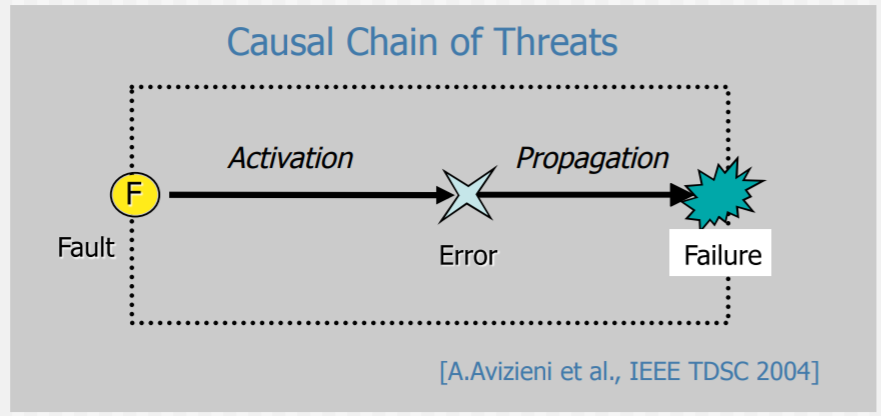
\includegraphics[scale=0.5]{../DokumenSkripsi/gambar/fault}
	\centering
	\caption{Rantai ancaman.}
\end{figure}
\begin{figure}
	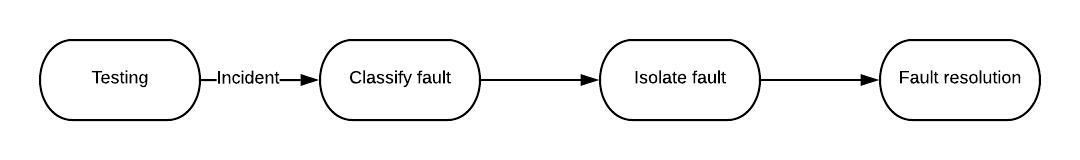
\includegraphics[scale=1.0]{../DokumenSkripsi/gambar/cycle2}
	\centering
	\caption{Siklus hidup pengujian.}
\end{figure}
Gambar 2 menggambarkan model siklus hidup untuk pengujian. Perhatikan bahwa, dalam fase pengembangan, tiga peluang muncul untuk membuat \textit{error}, yang menghasilkan \textit{fault} yang dapat menyebar melalui proses \textit{development}. Langkah resolusi \textit{fault} adalah kesempatan lain untuk \textit{error} (dan \textit{fault} baru). Ketika suatu perbaikan menyebabkan perangkat lunak yang sebelumnya benar untuk berperilaku salah, perbaikannya kurang.

Dari urutan \textit{term} ini, dapat dilihat bahwa \textit{test case} menempati posisi sentral dalam pengujian. Proses pengujian dapat dibagi lagi menjadi langkah-langkah terpisah: \textit{test planning, test case development}, menjalankan \textit{test case}, dan mengevaluasi hasil pengujian.Untuk \textit{test case} ada tiga pendekatan mendasar digunakan untuk mengidentifikasi \textit{test case}, yaitu:
\begin{itemize}
	\item \textit{Specification-Based/Black-box}
	\item \textit{Code-Based/White-box}
	\item \textit{Grey-box}
\end{itemize} 


\subsection*{\textit{Specification-Based/Black-box Testing}}
Alasan bahwa pengujian berbasis spesifikasi pada awalnya disebut \textit{functional testing} adalah bahwa setiap program dapat dianggap sebagai fungsi yang memetakan nilai dari domain input ke nilai dalam rentang outputnya. Gagasan ini umumnya digunakan dalam \textit{engineering}, ketika suatu sistem dianggap sebagai \textit{black box}. Ini mengarah pada istilah sinonim lainnya — pengujian \textit{black-box}, di mana konten (implementasi) kotak hitam tidak diketahui, dan fungsi kotak hitam dipahami sepenuhnya dalam hal input dan outputnya (lihat Gambar 3). Sering kali, pengujian beroperasi sangat efektif dengan pengetahuan \textit{black box}; pada kenyataannya, ini adalah pusat orientasi objek. Sebagai contoh, kebanyakan orang berhasil mengoperasikan mobil dengan hanya pengetahuan "\textit{black box}".
\begin{figure}[h!]
	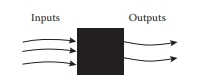
\includegraphics[scale=1.0]{../DokumenSkripsi/gambar/blackbox}
	\centering
	\caption{Engineer’s black box.}
\end{figure}

Dengan pendekatan berbasis spesifikasi untuk menguji identifikasi kasus, satu-satunya informasi yang digunakan adalah spesifikasi perangkat lunak. Oleh karena itu, \textit{test case} memiliki dua keunggulan berbeda: 
\begin{enumerate}
\item Tidak tergantung pada bagaimana perangkat lunak diimplementasikan, jadi jika implementasi berubah, \textit{test case} masih berguna.
\item Pengembangan \textit{test case} dapat terjadi secara paralel dengan implementasi, sehingga mengurangi keseluruhan interval pengembangan proyek.
\end{enumerate} 
Di sisi negatif, kasus uji berbasis spesifikasi sering mengalami dua masalah, redudansi yang signifikan ada di antara kasus uji, dan diperparah oleh kemungkinan kesenjangan perangkat lunak yang tidak diuji.

Gambar 4 menunjukkan hasil \textit{test case} yang diidentifikasi oleh dua metode berbasis spesifikasi. Metode A mengidentifikasi serangkaian kasus uji yang lebih besar daripada metode B. Perhatikan bahwa, untuk kedua metode, rangkaian kasus uji sepenuhnya terkandung dalam rangkaian perilaku tertentu. Karena metode berbasis spesifikasi didasarkan pada perilaku yang ditentukan, sulit untuk membayangkan metode ini mengidentifikasi perilaku yang tidak ditentukan.
\begin{figure}
	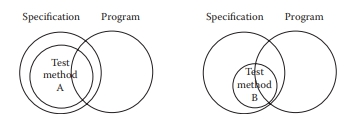
\includegraphics[scale=1.2]{../DokumenSkripsi/gambar/compareAB}
	\centering
	\caption{Comparing specification-based test case identification methods}
\end{figure}
\textit{Code-Based/White-box Testing} adalah pendekatan mendasar lainnya untuk menguji \textit{test case}. Untuk membandingkannya dengan pengujian \textit{black box}, kadang-kadang disebut pengujian \textit{white box} (atau bahkan \textit{clear box}). Metafora \textit{clear box} mungkin lebih tepat karena perbedaan mendasar adalah bahwa implementasi (\textit{black box}) diketahui dan digunakan untuk mengidentifikasi \textit{test case}. Kemampuan untuk "melihat ke dalam" \textit{black box} memungkinkan tester untuk mengidentifikasi \textit{test case} berdasarkan bagaimana fungsi tersebut benar-benar dijalankan.

\subsection*{\textit{Code-Based/White-box Testing}}
Pengujian berbasis kode telah menjadi subjek dari beberapa teori yang cukup kuat. Dengan konsep-konsep ini, tester dapat dengan ketat menggambarkan dengan tepat apa yang akan diuji. Karena dasar teorinya yang kuat, pengujian berbasis kode cocok untuk menjadi definisi dan penggunaan \textit{test coverage metrics}. \textit{Test coverage metrics} menyediakan cara untuk secara eksplisit menyatakan sejauh mana \textit{item} perangkat lunak telah diuji, dan ini pada gilirannya membuat manajemen pengujian lebih jelas.
\begin{figure}[h!]
 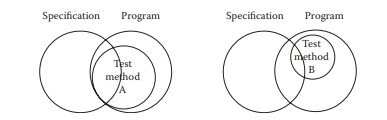
\includegraphics[scale=1.2]{../DokumenSkripsi/gambar/compareAB-whitebox}
 \centering
 \caption{Comparing code-based test case identification methods.}
\end{figure}
Gambar 5 menunjukkan hasil \textit{test case} yang diidentifikasi oleh dua metode berbasis kode. Seperti sebelumnya, metode A mengidentifikasi satu set kasus uji yang lebih besar daripada metode B. Apakah satu set kasus uji yang lebih besar tentu lebih baik? Ini adalah pertanyaan yang bagus, dan pengujian berbasis kode menyediakan cara-cara penting untuk mengembangkan jawaban. Perhatikan bahwa, untuk kedua metode, himpunan kasus uji sepenuhnya terkandung dalam himpunan perilaku yang diprogram. Karena metode berbasis kode didasarkan pada program, sulit membayangkan metode ini mengidentifikasi perilaku yang tidak diprogram. Sangat mudah untuk membayangkan, bagaimanapun, bahwa serangkaian kasus uji berbasis kode relatif kecil sehubungan dengan perilaku lengkap yang diprogram. 

\section*{\textit{Unit Testing}}
Tahap paling dalam pada pengujian perangkat lunak adalah \textit{unit testing}.Dalam \textit{unit testing}, kita menguji setiap unit kode secara individu, biasanya sebuah \textit{method}, dalam isolasi untuk melihat apakah jika diberikan suatu kondisi tertentu, apakah respons yang didapat akan sama dengan yang diharapkan (lihat Gambar 7). Memecah pengujian ke tingkat dasar memberi keyakinan bahwa setiap bagian dari aplikasi akan berperilaku seperti yang diharapkan dan memungkinkan untuk menutupi kasus di mana hal yang tidak terduga terjadi dan dapat ditangani dengan cara yang tepat.
\begin{figure}[h!]
	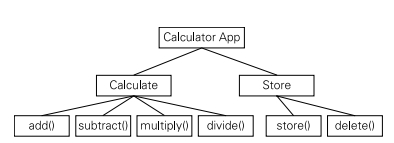
\includegraphics[scale=1.5]{../DokumenSkripsi/gambar/unittest}
	\centering
	\caption{Contoh struktur aplikasi yang menunjukkan kelas dan method. Method adalah "unit" yang akan diuji.}
\end{figure}

Pada contoh diatas, \textit{method} yang disorot adalah unit individual dari aplikasi ini yang perlu diuji.\textit{Method} pada kelas \textit{Calculator} berfungsi seperti yang diharapkan, maka kita yakin bahwa fitur-fitur aplikasi \textit{Calculator} tersebut telah berjalan sesuai harapan.

Misalnya, kita ingin menguji apakah hasil dari \textit{method} dengan dua angka benar-benar menambahkannya untuk menghasilkan jumlah yang benar. Memecah kode menjadi \textit{unit-unit} ini membuat proses pengujian lebih mudah. Saat berurusan dengan \textit{unit} kecil dari sebuah aplikasi, kita memiliki pemahaman yang jelas tentang cara kerja unit tersebut dan hal-hal yang memungkinkan untuk salah pada potongan kode tertentu, sehingga memungkinkan untuk menutupi \textit{unit} dengan tes yang sesuai.

Selain itu, saat melakukan pengujian dengan cara ini biasanya jelas jika kita telah memecah kode menjadi unit-unit. Jika harus menulis banyak tes berbeda untuk mencakup semua kemungkinan berbeda yang dapat dilalui \textit{method} ini, \textit{method} tersebut mungkin terlalu besar dan harus dipertimbangkan untuk melakukan \textit{refactoring} menjadi dua metode atau lebih dengan tanggung jawab yang sama. Sebaliknya, mungkin ada kasus di mana \textit{method} terlalu sederhana dan dapat dikombinasikan dengan beberapa fungsi lain untuk membuat \textit{method} yang lebih berguna. Sebagai seorang \textit{programmer} yang berpengalaman, kita harus mulai merasakan metode mana yang yang sudah "berukuran" baik dan mana yang tidak. Sepuluh baris sering merupakan aturan praktis yang baik untuk diikuti. Sebagai programmer yang baik, kita harus berusaha untuk memberikan kode yang paling mudah dibaca.

Tes yang ditulis adalah cerita yang menjelaskan kode dari sebuah program. Apa yang ingin dibaca atau dilihat ketika pertama kali membaca kode dan mencoba memahami apa fungsinya? Konvensi penamaan variabel yang jelas, ringkas, nama kelas, nama file, dan tes dapat membantu membuat kode lebih  mudah dipelihara untuk orang lain.

\section*{\textit{Behaviour-Driven Development}}
Behavior-Driven Development (BDD) adalah seperangkat praktik rekayasa perangkat lunak yang dirancang untuk membantu tim membangun dan memberikan perangkat lunak yang lebih bernilai dan berkualitas lebih cepat. Ini mengacu pada \textit{agile} dan \textit{lean practices} termasuk, khususnya, \textit{Test-Driven Development} (TDD) dan \textit{Domain-Driven Design} (DDD). Tetapi yang paling penting, BDD menyediakan bahasa umum berdasarkan kalimat-kalimat sederhana dan terstruktur yang diekspresikan dalam bahasa Inggris (atau dalam bahasa asli para pemangku kepentingan) yang memfasilitasi komunikasi antara anggota tim proyek dan pemangku kepentingan bisnis.

Untuk lebih memahami cara kerja BDD, dengan BDD yang hasil pengembangan dari TDD, kita harus membahas sedikit tentang TDD. Test-Driven Development (TDD) adalah praktik pengembangan yang menggunakan \textit{unit test} untuk menentukan, merancang, dan memverifikasi kode yang akan ditulis. Sebelum menerapkan fungsionalitas, pengembang menulis \textit{unit test} yang sengaja digagalkan untuk menunjukkan bagaimana fungsi ini seharusnya bekerja. Pada saat yang sama, pengujian gagal ini juga membuktikan bahwa implementasi saat ini belum mendukung fungsionalitas yang baru. Baru setelah itu pengembang menulis kode program. Setelah \textit{unit testing} berlalu, pengembang tahu bahwa fungsionalitas telah berhasil diimplementasikan. Pada tahap ini, mereka dapat meninjau kode mereka untuk merapikan dan menyempurnakan desain.

BDD pada awalnya dirancang sebagai versi perbaikan TDD. BDD awalnya ditemukan oleh Dan North pada awal hingga pertengahan 2000-an sebagai cara yang lebih mudah untuk mengajar dan mempraktikkan Test-Driven Development (TDD). TDD, ditemukan oleh Kent Beck pada awal munculnya \textit{Agile Development}, itu adalah teknik efektif yang menggunakan \textit{unit test} untuk menentukan, merancang, dan memverifikasi kode program.

Ketika pengguna TDD perlu mengimplementasikan fitur, mereka terlebih dahulu menulis tes gagal yang menjelaskan, atau menentukan fitur itu. Selanjutnya, mereka menulis kode yang cukup untuk lulus melakukan tes kode. Akhirnya, mereka memperbaiki kode untuk membantu memastikan bahwa kode itu akan mudah dirawat (lihat gambar 6). Teknik sederhana namun kuat ini mendorong pengembang untuk menulis kode yang lebih bersih, dirancang lebih baik, lebih mudah dirawat dan menghasilkan jumlah kecacatan kode yang jauh lebih rendah.

\begin{figure}
	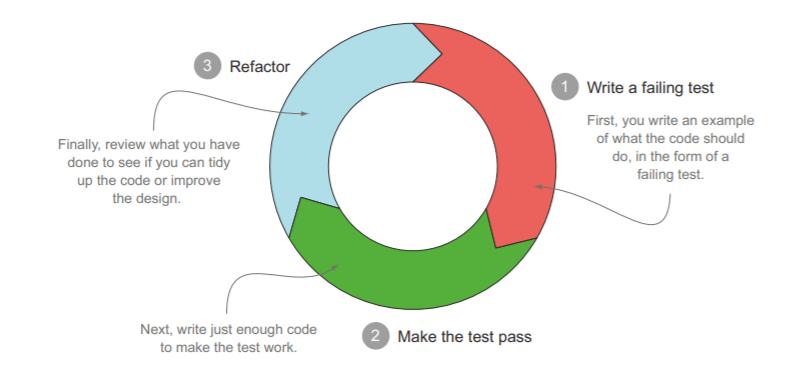
\includegraphics[scale=1.2]{../DokumenSkripsi/gambar/bdd}
	\centering
	\caption{Test-Driven Development three-phase cycle}
\end{figure}
Terlepas dari kelebihannya, banyak orang masih kesulitan mengadopsi dan menggunakan TDD secara efektif. Pengembang sering mengalami kesulitan mengetahui di mana harus memulai atau tes apa yang harus mereka tulis selanjutnya. Terkadang TDD dapat menyebabkan pengembang menjadi terlalu fokus pada detail, kehilangan gambaran yang lebih luas tentang tujuan bisnis yang seharusnya mereka terapkan. Beberapa tim juga menemukan bahwa sejumlah besar \textit{unit test} dapat menjadi sulit untuk dipertahankan karena ukuran proyek bertambah.

Faktanya, banyak \textit{unit testing} tradisional, ditulis dengan atau tanpa TDD, secara erat digabungkan dengan implementasi kode tertentu. Mereka fokus pada metode atau fungsi yang mereka uji, bukan pada apa yang harus dilakukan kode dalam  bisnis \textit{term}.

BDD juga berfungsi dengan baik untuk \textit{requirements analysis}. Bekerja dengan rekan analis bisnis Chris Matts, North mulai menerapkan apa yang telah ia pelajari ke ruang \textit{requirements analysis}. Eric Evans memperkenalkan gagasan \textit{Domain-Driven Design}, yang mempromosikan penggunaan bahasa yang dapat dimengerti dimanapun agar dapat dipahami oleh  orang dari sisi bisnis untuk menggambarkan dan memodelkan suatu sistem. Visi North dan Matts adalah untuk menciptakan bahasa untuk dimengerti oleh siapapun yang dapat digunakan oleh analis bisnis untuk mendefinisikan persyaratan secara jelas, dan itu juga dapat dengan mudah diubah menjadi \textit{acceptance tests} yang otomatis. Untuk mengimplementasikan visi ini, mereka mulai mengekspresikan \textit{acceptance criteria} untuk \textit{user stories} dalam bentuk contoh yang terstruktur, yang dikenal sebagai "skenario," seperti ini:\\
\texttt{\textbf{Given} a customer has a current account \\
\textbf{When} the customer transfers funds from this account to an overseas account\\
\textbf{Then} the funds should be deposited in the overseas account\\
\textbf{And} the transaction fee should be deducted from the current account\\}
\textit{Keyword} dari skenario yaitu \textit{Given,When} dan \textit{Then}, makna dari masing-masing \textit{keyword} ialah: 
\begin{itemize}
 \item \textit{Given} menjelaskan prekondisi untuk skenario dan mempersiapkan \textit{environment} untuk tes.
 \item \textit{When} menjelaskan tindakan yang sedang dilakukan pada tes.
 \item \textit{Then} menjelaskan hasil yang diharapkan.
 \item \textit{And} dan \textit{But} bisa digunakan untuk menggabungkan beberapa dari \textit{keyword} diatas.
\end{itemize}

Pemilik bisnis dapat dengan mudah memahami skenario yang ditulis seperti ini. Ini memberikan tujuan yang jelas dan objektif untuk setiap cerita dalam hal apa yang perlu dikembangkan dan apa yang perlu diuji.

Notasi ini akhirnya berkembang menjadi bentuk yang umum digunakan, dan sering disebut sebagai Gherkin. Dengan \textit{tools} yang tepat, skenario yang ditulis dalam formulir ini dapat diubah menjadi \textit{acceptance criteria} yang otomatis dan dapat dieksekusi secara otomatis juga kapanpun diperlukan. 

Ketika sebuah tim yang mempraktikkan BDD memutuskan untuk mengimplementasikan sebuah fitur, mereka bekerja bersama dengan pengguna dan \textit{stakeholders} lainnya untuk mendefinisikan \textit{user stories} dan skenario tentang apa yang diharapkan oleh pengguna untuk diberikan oleh fitur ini. Secara khusus, para pengguna membantu mendefinisikan sekumpulan contoh konkret yang menggambarkan \textit{key outcome} dari fitur tersebut. (Lihat Gambar 8)
\begin{figure}
	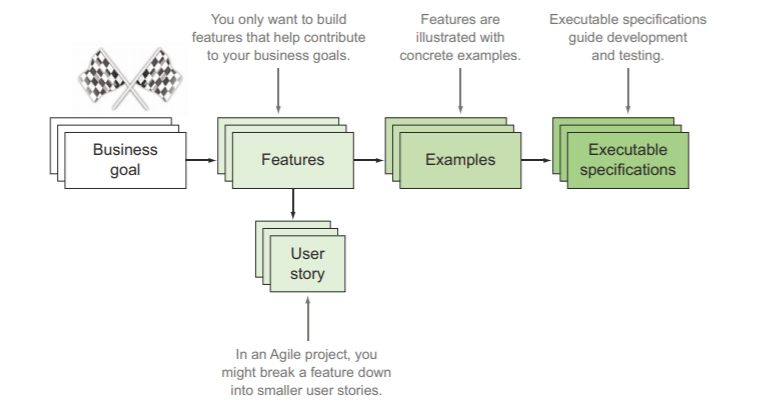
\includegraphics[scale=1.2]{../DokumenSkripsi/gambar/skenario}
	\centering
	\caption{Examples play a primary role in BDD, helping everyone understand the
requirements more clearly}
\end{figure}

\textit{Examples} ini menggunakan kosakata umum dan dapat dengan mudah dipahami oleh pengguna dan anggota tim pengembang. Mereka biasanya diekspresikan menggunakan Notasi \textit{Given} ... \textit{When} ... \textit{Then} yang sama seperti contoh tadi diatas. Misalnya, contoh sederhana yang menggambarkan fitur "\textit{Transfer funds between a client’s accounts}" mungkin terlihat seperti ini:\\
\texttt{Scenario: Transferring money to a savings account\\
 Given I have a current account with 1000.00\\
 And I have a savings account with 2000.00\\
 When I transfer 500.00 from my current account to my savings account\\
 Then I should have 500.00 in my current account\\
 And I should have 2500.00 in my savings account\\}
 
\textit{Examples} memainkan peran utama dalam BDD, hanya karena mereka adalah cara yang sangat efektif untuk mengkomunikasikan persyaratan yang jelas, tepat, dan tidak ambigu. Spesifikasi yang ditulis dalam bahasa alami, ternyata, merupakan cara komunikasi yang sangat buruk, karena ada begitu banyak ruang untuk ambiguitas, asumsi, dan kesalahpahaman. Contohnya adalah cara yang bagus untuk mengatasi keterbatasan ini dan mengklarifikasi persyaratan. \textit{Examples} adalah cara yang bagus untuk mengatasi keterbatasan ini dan mengklarifikasi persyaratan.

\section*{\textit{Code Coverage}}
\textit{Code Coverage} adalah metrik yang digunakan untuk mengkarakterisasi tingkat di mana beberapa  kode aplikasi telah dieksekusi setelah dilakukannya tes. Ini dihitung dengan hasil berbentuk persentase, dihitung dengan pembagian $\frac{Code{\tiny exec}}{Code{\tiny region}}$, menunjukkan jumlah kode sumber yang sudah dieksekusi (Code{\tiny exec}) berkenaan dengan jumlah total kode sumber yang harus dilakukan (Code{\tiny region}).

Semakin tinggi \textit{code coverage}-nya, semakin besar jumlah kode yang dikerjakan selama eksekusi pengujian sehubungan dengan \textit{region} kode yang diuji. Meskipun telah ditunjukkan bahwa cakupan kode yang tinggi tidak selalu berarti deteksi \textit{bug} yang tinggi. Namun, tidak mungkin untuk mengatakan apapun tentang area kode yang tidak pernah dijalankan. Dengan demikian, \textit{code coverage} yang digunakan sebagai relatif \textit{measure} berfungsi sebagai indikator yang cocok untuk pengujian yang baik.

Secara umum, \textit{code coverage} dilakukan dengan menginstruksikan kode aplikasi dan kemudian memperoleh data cakupan dari bagian instrumentasi. Ada beberapa alat yang menyediakan informasi seperti itu, misalnya, JaCoCo4. Namun, dalam beberapa konteks, peneliti tidak diizinkan untuk melakukan instrumentasi, karena pengujian tidak dilakukan di tingkat pengembangan. Dalam kasus seperti itu, hanya mungkin untuk melakukan proses pemantauan yang tidak perlu memodifikasi aplikasi yang sudah dikompilasi. Untuk Android, kami menggunakan ddmlib5 \textit{tracer} untuk melihat ketika metode dipanggil saat melakukan eksekusi \textit{test case}.

Ada beberapa kriteria untuk melakukan \textit{code coverage}, yaitu :
\begin{itemize}
\item \textit{Statement Coverage} --- Mengeksekusi pernyataan program secara individual dan mengamati semua hasilnya. \textit{Statement coverage} 100\% berarti semua pernyataan telah dieksekusi sedikitnya satu kali.
\item \textit{Branch Coverage} --- Mengeksekusi \textit{branch} yang ada pada \textit{statement} program. \textit{Branch coverage} 100\% berarti semua branch yang ada di program sudah berhasil dieksekusi sedikitnya satu kali.
\item \textit{Condition coverage} --- Mengeksekusi semua kondisi yang ada pada statement kode program.
\textit{Condition coverage} 100\% berarti semua kemungkinan kombinasi nilai dari kondisi yang mempengaruhi jalur telah dieksplorasi dalam  pengujian.
\item \textit{Branch\&Condition Coverage} --- Gabungan dari \textit{branch coverage} dan juga \textit{condition coverage}.
\item \textit{Path Coverage} --- Mengeksekusi semua kemungkinan kombinasi pada kode program, bisa dibilang ini gabungan semua dari kriteria sebelumnya. \textit{Path coverage} 100\% berarti semua kode pada program sudah berhasil dieksekusi dan semua kemungkinan kode program sudah berhasil dilewati setidaknya satu kali.
\end{itemize}
		
		\item \textbf{Melakukan eksplorasi perangkat lunak}\\
		{\bf Status :} Ada sejak rencana kerja skripsi.\\
		{\bf Hasil :} Melakukan eksplorasi perangkat lunak sudah dilakukan dengan membaca buku tentang behaviour-driven development, behaviour specification dan melihat cara kerja perangkat lunak yang menggunakan BDD sebagai dasar sistemnya.
		
Perangkat lunak yang menggunakan BDD sebagai dasar rata-rata menggunakan format Gherkin yang digunakan untuk merancang sebuah sistem, dimana Gherkin dirancang/dibuat oleh \textit{stakeholder} dan dari situ tim pengembang akan membuat sistem berpatokan dari Gherkin yang sudah dibuat oleh \textit{stakeholder}.

Perangkat lunak akan menerima input teks dengan format Gherkin sebagai berikut:
\begin{itemize}
 \item \textit{\textbf{Given}} menjelaskan prekondisi untuk skenario dan mempersiapkan \textit{environment} untuk tes.
 \item \textit{\textbf{When}} menjelaskan tindakan yang sedang dilakukan pada tes.
 \item \textit{\textbf{Then}} menjelaskan hasil yang diharapkan.
 \item \textit{\textbf{And}} dan \textit{\textbf{But}} bisa digunakan untuk menggabungkan beberapa dari \textit{keyword} diatas.
\end{itemize}
Dari \textit{keywords} yang ditebalkan tersebut akan digunakan sebagai kunci oleh perangkat lunak untuk melakukan sesuatu. Contoh dengan skenario:\\
\texttt{\textbf{Scenario}: Buying a single product\\
\textbf{Given} there is a Playstation 4, which cost \$250\\
\textbf{When} I add the Playstation 4 to the basket\\
\textbf{Then} I should have 1 product in the basket\\
\textbf{And} the overall basket price should be\$250\\}
\textit{Given} pada skenario diatas merupakan parameter dari sebuah \textit{method} pada perangkat lunak, \textit{When} disitu merupakan cara kerja/nama \textit{method} (karena nama \textit{method} melambangkan isi dari \textit{method} itu sendiri),  \textit{Then} merupakan hasil yang diharapkan dari \textit{method} dan yang terakhir \textit{And} tambahan untuk hasil \textit{Then}. 
		\item \textbf{Menganalisis kebutuhan perangkat lunak}\\
		{\bf Status :} Ada sejak rencana kerja skripsi.\\
		{\bf Hasil :} Menganalisis kebutuhan perangkat lunak sudah dilakukan dengan mencari berbagai program pengujian perangkat lunak dan \textit{tools} apa yang digunakan. Buku yang digunakan untuk referensi yaitu \textit{Beginning HTML with CSS and XHTML: Modern Guide and Reference, PHP and MySQL Manual,} dan \textit{CodeIgniter 1.7 Professional 
Development}

\section*{HTML}
HyperText Markup Language (HTML) adalah bahasa pengkodean komputer yang digunakan untuk mengubah teks biasa menjadi teks aktif untuk ditampilkan dan digunakan di web dan juga untuk memberikan teks biasa, tidak terstruktur, jenis struktur yang diandalkan manusia untuk membacanya. Tanpa semacam struktur yang digunakan pada html, teks biasa hanya akan berjalan bersama tanpa apapun untuk membedakan satu untaian kata dari yang lain.

HTML terdiri dari penanda yang dikodekan yang disebut \textit{tag} yang mengelilingi dan membedakan bit teks, yang menunjukkan fungsi dan tujuan dari teks yang diberi tag. Tag tertanam secara langsung dalam dokumen teks biasa di mana mereka dapat diinterpretasikan oleh perangkat lunak komputer. Tag HTML menunjukkan sifat sebagian konten dan memberikan informasi penting tentangnya. Tag berdiri sendiri tidak ditampilkan dan berbeda dari konten yang sebenarnya mereka sampaikan.

\section*{PHP}
PHP (PHP Hypertext Pre-processor) adalah bahasa scripting yang disematkan HyperText Markup Language (HTML). Tujuan dari bahasa ini adalah untuk memungkinkan pembangunan halaman Web dinamis dengan cepat dan mudah. PHP bekerja bersama dengan server web dan dapat digunakan dengan berbagai sistem operasi, termasuk Microsoft Windows dan UNIX.

PHP tertanam dalam dokumen HTML dengan tag awal dan akhir khusus yang memungkinkan untuk keluar dan masuk dari PHP. Ini memberikan waktu tampilan halaman yang cepat, keamanan tinggi dan transparansi bagi pengguna. Dengan PHP kita dapat memperoleh semua yang dapat dicapai dengan menulis aplikasi terpisah, seperti membuat halaman web yang dinamis, pemrosesan formulir dan penanganan file.

Sintaks PHP mirip dengan bahasa pemrograman C, C ++ dan Java. Jika  memiliki pengetahuan tentang bahasa-bahasa ini, maka akan menemukan bahwa bahasa PHP sangat akrab. PHP sederhana dan mudah untuk dipahami, jangan takut untuk mempelajari bahasa ini.

Salah satu fasilitas terpenting dan terkuat dari PHP adalah kemampuannya untuk berinteraksi dengan berbagai macam basis data. Lebih dari 20 basis data yang berbeda saat ini didukung, memungkinkan pengembang PHP untuk membuat halaman Web dengan basis data yang mudah. 

CodeIgniter adalah \textit{framework} aplikasi web yang bersifat \textit{open source} untuk bahasa PHP. CodeIgniter memiliki banyak fitur yang membuatnya menonjol dari \textit{framework} lainnya. Tidak seperti beberapa \textit{framework} PHP lain yang, dokumentasinya sangat menyeluruh dan lengkap, mencakup setiap aspek \textit{framework}. 

Di sisi pemrograman, CodeIgniter kompatibel dengan PHP4 dan PHP5, sehingga akan berjalan di sebagian besar web host di luar sana. CodeIgniter juga menggunakan pola desain \textit{Model View Controller} (MVC), yang merupakan cara untuk mengatur aplikasi Anda menjadi tiga bagian berbeda: \textit{model} — lapisan abstraksi basis data, \textit{view} — file tampilan depan, dan \textit{control} — logika bisnis aplikasi. Pada intinya, CodeIgniter juga memanfaatkan pola desain \textit{Singleton} secara ekstensif. Ini adalah cara untuk memuat kelas sehingga jika mereka dipanggil beberapa kali, instance kelas yang sama akan dikembalikan. Ini sangat berguna untuk koneksi basis data, karena hanya ingin satu koneksi setiap kali kelas digunakan.


		\item \textbf{Membuat rancangan desain antarmuka perangkat lunak.}\\
		{\bf Status :} Ada sejak rencana kerja skripsi.\\
		{\bf Hasil :}Membuat rancangan desain antarmuka perangkat lunak sudah dilakukan dengan menggunakan HTML dan CSS.
		\begin{figure}[h!]
			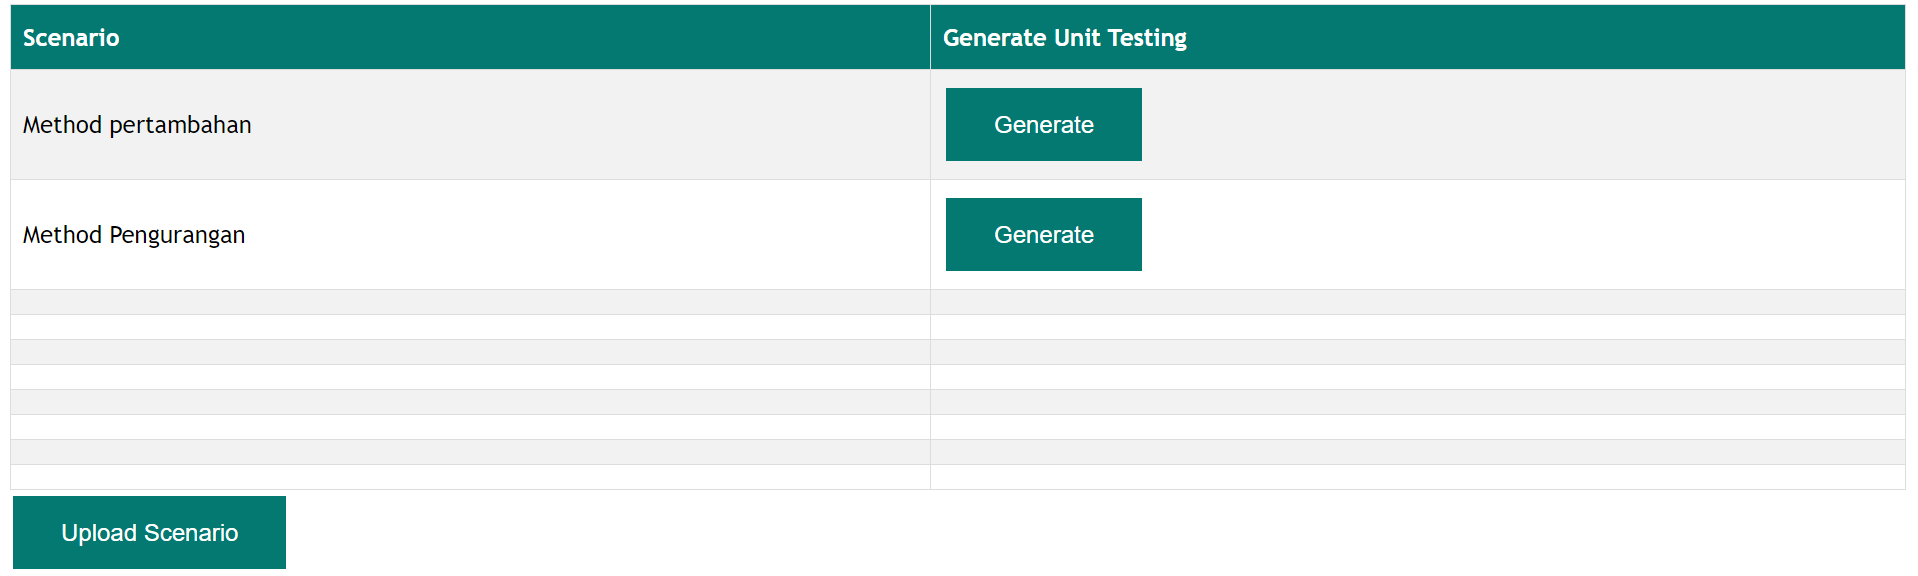
\includegraphics[scale=0.45]{../DokumenSkripsi/gambar/uiFix}
			\centering
			\caption{Tampilan antarmuka perangkat lunak}
		\end{figure}
		Dapat dilihat pada gambar 9 terdapat tabel yang berisikan 2 kolom. Tabel tersebut berfungsi untuk menampung unit testing yang akan diuji jika tombol pada kolom 2 ditekan pada method yang akan diuji. Dibawah tabel tersebut terdapat tombol untuk melakukan \textit{upload} unit testing yang berupa file berisi skenario dengan format Gherkin. Setelah file tersebut diunggah maka unit testing tersebut akan tertera pada tabel tersebut.
		
		\item \textbf{Mempelajari \textit{Framework} PHPUnit.}\\
		\textbf{Status :} Ada sejak rencana kerja skripsi.\\
		\textbf{Hasil : } Sudah mempelajari cara kerja PHPUnit agar dapat diimplementasikan pada perangkat lunak yang akan dibangun. Mencari dari berbagai sumber untuk dapat memahami secara penuh bagaimana PHPUnit bekerja dan kendala apa saja yang bisa didapati ketika menggunakan \textit{framework} ini, sehingga ketika perangkat lunak akan dibangun sudah bisa meminimalisir masalah apa saja yang bisa didapati dengan begitu pembangungan perangkat lunak akan minim akan masalah. Sumber utama untuk mempelajari PHPUnit saya membaca dokumen dari website utama PHPUnit (\textit{https://phpunit.de})
		
		\item \textbf{Melakukan analisis masalah.}\\
		\textbf{Status :}Ada sejak rencana kerja skripsi.\\
		\textbf{Hasil :} Pada pengembangan perangkat lunak ada beberapa tahapan yang harus dilakukan agar akhirnya perangkat lunak bisa digunakan oleh pengguna tanpa lagi ada nya error. Tahapan-tahapan tersebut yaitu ada \textit{analysis, design, coding, testing, installation, dan maintenance}. \textit{Testing}/Pengujian perangkat lunak adalah proses untuk mencari kesalahan pada setiap komponen perangkat lunak, mencatat hasilnya, mengevaluasi setiap aspek pada setiap komponen dan mengevaluasi fitur-fitur dari perangkat lunak yang akan dikembangkan. Dengan adanya pengujian ini, perangkat lunak akan di periksa seluruh bagian nya hingga dipastikan tidak ada lagi \textit{error} dan akhirnya bisa digunakan oleh pengguna. Pengujian perangkat lunak ada beberapa tahapan yaitu \textit{unit test, integration test, system test, dan acceptance test.}
		
		Disini akan membahas lebih dalam cara kerja \textit{unit testing}. \textit{Unit Testing} merupakan tahapan pertama dari pengujian perangkat lunak, dimana melakukan pengujian pada setiap komponen individu sebuah perangkat lunak dan melakukan verifikasi apakah kode tersebut berjalan sesuai yang diinginkan atau tidak. Salah satu teknik pengembangan perangkat lunak yaitu \textit{Behaviour-driven development} (BDD), dimana BDD merupakan pengembangan dari metode \textit{Test-driven development}(TDD) untuk menyelesaikan masalah yang ada pada TDD, BDD adalah seperangkat praktik rekayasa perangkat lunak yang dibuat untuk membantu tim membangun dan memberikan perangkat lunak yang memfasilitasi komunikasi antara anggota tim proyek dan pemangku kepentingan bisnis. BDD berpatokan pada keinginan \textit{stakeholder} untuk mengembangkan programnya. Untuk mencapai kesepakatan antara pengembang dan \textit{stakeholder}, maka dibutuhkan \textit{language} untuk menspesifikasikan \textit{behaviour} sebuah sistem agar kedua pihak paham, \textit{language} tersebut bisa berupa \textit{scenario}, yang dimana \textit{scenario} tersebut berisi \textit{Context/Starting state}, \textit{Event}, \textit{Outcome}.
		
		Pengembang akan menjadikan skenario sebagai patokan dasar bekerjanya suatu sistem, dan akan melakukan pengujian berbasis skenario. Pengujian dilakukan untuk memastikan bahwa sistem sudah bekerja sesuai apa yang \textit{stakeholder} harapkan, dan jika \textit{scenario} berhasil dilakukan, maka sistem sudah siap untuk digunakan.
		
		Untuk mewujudkan sistem seperti apa yang diinginkan oleh \textit{stakeholder}, pada skripsi ini skenario yang akan digunakan yaitu seperti pada bab 2 sudah disebutkan yaitu skenario berformat Gherkin, Gherkin ini sudah biasa digunakan ketika menggunakan metode BDD. Pada skripsi ini Gherkin diterapkan dengan menggunakan \textit{keyword-keyword}, ketika \textit{keyword} tersebut ditemukan pada skenario yang digunakan, maka pada \textit{code} akan di-\textit{setting} untuk melakukan sesuatu. 
		
		Pada skripsi ini format \textit{unit testing} yang akan dihasilkan yaitu berformat php, lebih tepat nya yang ingin dihasilkan oleh skripsi ini yaitu \textit{auto-generate unit testing} menggunakan skenario Gherkin, jadi ketika skenario Gherkin sudah diberikan oleh \textit{stakeholder}, skenario tersebut akan diproses menggunakan program yang akan dibangun pada skripsi ini agar menghasilkan sebuah \textit{unit testing} cukup hanya dengan skenario yang sudah diberikan oleh \textit{stakeholder}. \textit{Website} yang akan diuji menggunakan HTML dan PHP, dimana HTML disini digunakan untuk membuat tampilan \textit{website} dan php digunakan untuk \textit{logic} pada website ini. \textit{Website} yang digunakan disini yaitu bernama e-library, dimana \textit{website} e-library ini merupakan \textit{website} sistem informasi sederhana dimana pengguna bisa melihat buku apa saja yang ada dalam katalog buku dan meminjam nya(tapi belum diimplementasikan untuk fitur ini), pengguna bisa \textit{login} dan \textit{signup}, dan ada 2 tipe pengguna disini yaitu ada admin dan ada pengguna biasa. Sebelum website ini bisa digunakan untuk melakukan \textit{unit testing}, ada beberapa bagian pada \textit{logic website} yang menggunakan php harus disesuaikan sedikit agar \textit{unit testing} dapat diimplementasikan pada website ini, contohnya pada \textit{logic website} ini ada beberapa kode php yang diubah cara kerjanya agar dapat memenuhi syarat melakukan \textit{unit testing}, anggapannya kode php diubah sedikit menjadi \textit{Object-Oriented} dimana kode-kode php yang melakukan suatu fungsi pada fitur tertentu dimasukan kedalam \textit{method}, yang sebelumnya kode-kode tersebut tidak berada dalam \textit{method}, dan ada beberapa detail juga yang dilakukan agar \textit{unit testing} bisa dilakukan.
		
		Setelah \textit{website} dimodifikasi sedikit menjadi lebih  \textit{object-oriented} maka sudah bisa untuk diuji \textit{unit testing}, \textit{unit testing} disini menggunakan PHPUnit, dimana PHPUnit merupakan framework yang biasa digunakan pada bahasa PHP, metode yang akan banyak digunakan pada PHPUnit yaitu \textit{assertEquals}, dimana metode ini membutuhkan \textit{\textbf{actual result}} yaitu hasil yang didapatkan dari fitur yang dikeluarkan oleh \textit{website} e-library dan \textit{\textbf{expected result}} merupakan hasil yang diharapkan oleh \textit{stakeholder/developer} untuk dikeluarkan oleh sistem. Metode \textit{assertEquals} membandingkan \textit{actual result} dan \textit{expected result}, jika hasil kedua itu sama, maka \textit{unit testing} dianggap berhasil dan juga sebaliknya, jika hasil kedua nya tidak sama, maka \textit{unit testing} dianggap gagal karena hasil dari sistem dan dengan yang diinginkan \textit{stakeholder/developer} berbeda.
        
        
        \item \textbf{Merancang perangkat lunak tahap awal.}\\
        \textbf{Status :} Ada sejak rencana kerja skripsi.\\
        \textbf{Hasil :} \textit{Website} e-library yang akan diuji harus dimodifikasi agar bisa dilakukan \textit{unit testing}, walaupun yang ingin capai pada skripsi ini yaitu \textit{auto-generate unit testing} dari skenario Gherkin, tapi sebelum hal tersebut dilakukan, harus dipastikan bahwa \textit{unit testing} secara manual bisa juga dilakukan, maka untuk mengujinya unit testing dibuat terlebih dahulu menggunakan framework PHPUnit. Menguji seluruh fitur yang ada pada \textit{website} tersebut, dimana website e-library memiliki beberapa fitur utama yang akan diuji, yaitu:
        \begin{itemize}
            \item \textbf{addAdmin} : Fitur ini berguna bagi seorang admin untuk menambah admin baru.
            \item \textbf{addBook} : Fitur bagi admin untuk menambah buku baru pada katalog e-library.
            \item \textbf{login} : Login berguna bagi admin maupun user biasa untk mengakses berbagai fitur yang dimiliki \textit{website} e-library.
            \item \textbf{signup}: Fitur signup berguna untuk menambah pengguna pada database, agar pengguna dapat mengakses fitur \textit{website} e-library dengan signup terlebih dahulu setelah itu dapat login menggunakan akun yang sudah didaftarkan.
            \item \textbf{updateUser} : Fitur ini dapat digunakan baik oleh admin maupun pengguna biasa, dimana pengguna \textit{website} e-library dapat melakukan \textit{update} terhadap profil masing-masing.
        \end{itemize}
Setelah \textit{unit testing} berhasil dibuat dan ketika dicoba berhasil melakukan \textit{unit testing}, maka tahap selanjutnya yaitu mencari cara mengerjakan program yang akan dihasilkan pada skripsi ini, dengan menggunakan Gherkin, bisa memanfaatkan \textit{keyword-keyword} yang sudah disediakan dari Gherkin nya, dan bisa juga membuat patokan dengan \textit{keyword} baru, contoh keyword pada Gherkin yaitu ada \textbf{Given, When, And, Then} dan untuk skripsi ini, dapat juga menggunakan \textit{keyword} seperti:
\begin{itemize}
	\item \textbf{halaman}\\ dimana kata tersebut menandakan bahwa \textit{unit testing} yang akan dilakukan yaitu fitur yang melakukan pindah halaman setelah suatu event terjadi
	\item \textbf{tabel}\\ dimana kata tersebut menandak bahwa unit testing yang akan dilakukan yaitu menguji suatu fitur yang memasukan suatu data ke database
	\item \textbf{username}\\
	memasukan \textit{value} \textbf{username} yang pengguna \textit{input}
	\item \textbf{password}\\
	memasukan \textit{value} \textbf{password} yang pengguna \textit{input}
	\item \textbf{confirm password}\\
	memasukan \textit{value} \textbf{confirm password} yang pengguna \textit{input}
	\item \textbf{email}\\
	memasukan \textit{value} \textbf{email} yang pengguna \textit{input}
	\item \textbf{name}\\
	memasukan \textit{value} \textbf{name} yang pengguna \textit{input}
	\item \textbf{phone}\\
	memasukan \textit{value} \textbf{phone} yang pengguna \textit{input}
	\item \textbf{address}\\
	memasukan \textit{value} \textbf{address} yang pengguna \textit{input}
	\item \textbf{dan} \textit{value input} pengguna lainnya. 
\end{itemize}

Dengan sudah adanya \textit{unit testing} yang dibuat sebelum melakukan \textit{auto-generate unit testing} dengan menggunakan Gherkin, kode pada program yang akan dihasilkan bisa dibuat dengan berpatokan pada \textit{unit testing} yang sudah dihasilkan sebelumnya. \textit{Unit Testing} yang sudah jadi digunakan sebagai bayangan agar mempermudah ketika nanti membuat perangkat lunak, tidak  berpatok sepenuhnya terhadap \textit{unit testing} tersebut, untuk perangkat lunak yang akan dibangun, kasus nyata nya perangkat lunak akan berpatokan dengan skenario Gherkin yang sudah diberikan oleh \textit{stakeholder}, alur cara kerja perangkat lunak bisa dilihat seperti flowchart pada gambar 10:

\begin{figure}[h!]
			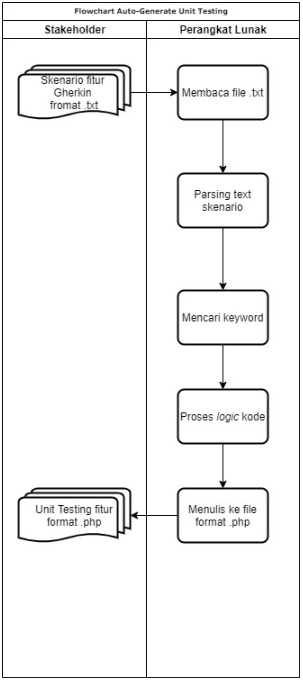
\includegraphics[scale=0.70]{../DokumenSkripsi/gambar/flowcharttesting}
			\centering
			\caption{Flowchart cara kerja perangkat lunak}
		\end{figure}

Dapat dilihat pada \textit{flowchart} pada gambar 10, inti alur cara kerja perangkat lunak yaitu dari skenario yang sudah diberikan oleh \textit{stakeholder} akan diproses oleh perangkat lunak hingga akhirnya menjadi suatu \textit{unit testing}, dari file text akan berubah menjadi suatu kode yang dapat digunakan untuk menguji suatu \textit{website}.

Alur dari cara kerja perangkat lunak dimulai dari skenario yang sudah diberikan dari \textit{stakeholder}, contoh skenario yang akan dipakai misalnya:

\texttt{Feature: loginVer\\
    Untuk menggunakan program\\
    Pengguna harus login terlebih dahulu\\
    Scenario: Login berhasil user\\
        Given Pengguna belum Login\\
        When Pengguna menekan tombol login\\
        And Pengguna mengisi username dengan dipo\\
        And Pengguna mengisi password dengan dipo\\
        Then Berhasil masuk ke halaman "Location:../pages/user/usr.php"}
     
Setelah mendapat skenario dari \textit{stakeholder}, maka perangkat lunak akan membaca dan melakukan \textit{parsing} setiap kata dari skenario tersebut, setelah mendapatkan setiap kata, make kata tersebut bisa didefinisikan mana kata yang merupakan \textit{keyword-keyword} yang akan menentukan cara kerja perangkat lunak nanti. Pada contoh skenario Gherkin di atas, kata yang sudah di \textit{bold keyword} yang akan digunakan pada perangkat lunak yang akan dikembangkan, contoh \textit{keyword} \textbf{tombol} pada kalimat \textbf{When}, dimana kata \textbf{When} menandakan \textit{event} yang sedang terjadi, maka bisa dianggap bahwa kata setelah \textbf{tombol} merupakan suatu fitur/\textit{method} yang ada pada \textit{website} e-library. Fitur \textit{login} membutuhkan \textbf{username} dan \textbf{password} agar bisa dilakukan \textit{unit testing}, maka pada skenario tersebut terdapat \textit{keyword} dari kedua kata tersebut, dan yang terakhir ada kata \textbf{Then}, untuk kalimat yang berawal \textbf{Then} menandakan bahwa tujuan akhir/hasil yang diharapkan dari fitur ini yaitu page \textit{website} akan berpindah yang asalnya homepage menjadi halaman user. Dapat dicontohkan dengan pseudocode:

if(kata[i]==”When”)

\hspace{5mm}if(kata[i]==”tombol”)

\hspace{10mm}\$method=kata[i+1];

menandakan \textbf{When} dan \textbf{tombol} sebagai \textit{keyword}, dan untuk \textit{keyword} \textbf{tombol} dapat dimasukan kata setelahnya (i+1 menandakan kata setelahnya) menjadikan kata tersebut fitur apa yang akan di generate menjadi \textit{unit testing}. 

if(kata[i]==”username”)

\hspace{5mm}	\$username=kata[i+2]; 

if(kata[i]==”password”)

\hspace{5mm}	\$password=kata[i+2]; 

Karena fitur login membutuhkan \textit{username} dan \textit{password}, maka butuh dimasukan juga ke suatu variabel (i+2 disini karena username dan password 2 kata setelah keyword) 

if(kata[i]==”Then”)

\hspace{5mm}	if(kata[i]==”halaman”)
	
\hspace{10mm}		if(\$method==”login”)
		
\hspace{15mm}			//menulis kode yang akan men generate kode unit testing dalam format php.

Disini \textit{keyword} \textbf{Then} menandakan bahwa hasil yang ingin dicapai sistem, didapatkan \textit{keyword} kedua yaitu \textbf{halaman} berarti tujuan akhir sistem yaitu pindah halaman, dan diperiksa untuk memastikan fitur mana yang ingin di \textit{generate} menjadi \textit{unit testing}, yaitu fitur \textit{login}, maka setelah itu sudah terdapat satu method \textit{unit testing} untuk \textit{login}. 

\begin{figure}[h!]
			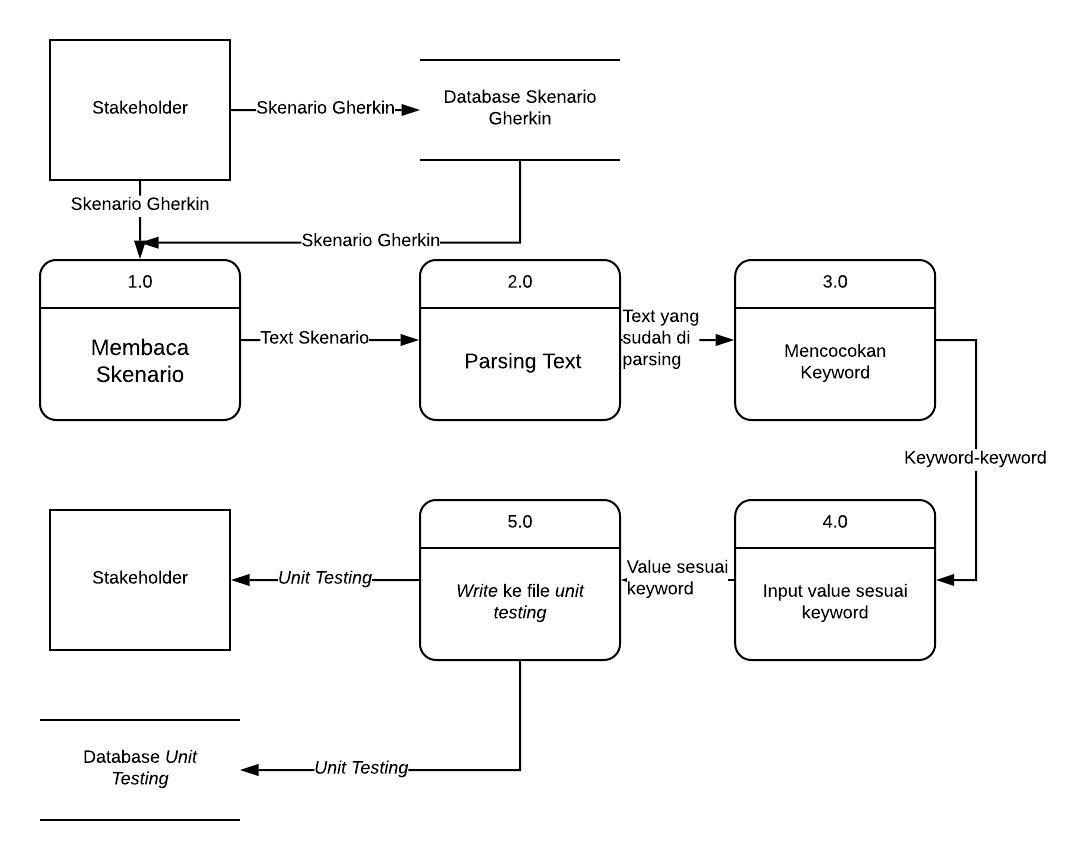
\includegraphics[scale=0.80]{../DokumenSkripsi/gambar/dfddiagram}
			\centering
			\caption{Diagram DFD cara kerja perangkat lunak}
		\end{figure}
		
Agar dapat lebih jelas melihat alur data \textit{input} dan \textit{output} nya, maka bisa dilihat dari diagram dfd pada gambar 11. \textit{Stakeholder} disini berguna sebagai pemberi skenario Gherkin, dimana nanti skenario tersebut akan menjadi rancangan untuk membuat \textit{unit testing}. Untuk lebih jelasnya dapat dilihat \textit{data dictionary} akan dijelaskan dengan \textit{data dictionary}:
\begin{center}
\begin{tabular}{ |l|l| } 
 \hline
 Process Name &  Membaca skenario\\ 
 \hline
 Process Number &  1.0 \\ 
 \hline
 Purpose &  Membaca skenario\\ 
 \hline
 Input Data Flows & Skenario Gherkin baik langsung dari stakeholder atau yang sudah ditempatkan di database \\
 \hline
 Output Data Flows & Text skenario yang sudah dapat diproses \\
 \hline
 Process Description & Membaca skenario yang diberikan oleh stakeholder agar bisa diproses lebih lanjut \\
 \hline
 Notes & File skenario Gherkin harus sesuai format agar proses berjalan lancar\\
 \hline
\end{tabular}
\end{center}

\begin{center}
\begin{tabular}{ |l|l| } 
 \hline
 Process Name &  Parsing Text\\ 
 \hline
 Process Number &  2.0 \\ 
 \hline
 Purpose & Melakukan parsing pada text \\ 
 \hline
 Input Data Flows & Text skenario Gherkin  \\
 \hline
 Output Data Flows & Text yang sudah di parsing \\
 \hline
 Process Description & Melakukan parsing text agar text bisa menjadi kumpulan kata-kata yang nantinya  \\
  & dapat diproses untuk mendapatkan keyword\\
 \hline
 Notes & Proses parsing ini merubah text menjadi kumpulan kata agar mempermudah mengakses\\
 &  setiap katanya, jika masih berupa kalimat akan sulit\\
 \hline
\end{tabular}
\end{center}

\begin{center}
\begin{tabular}{ |l|l| } 
 \hline
 Process Name & Mencocokan Keyword \\ 
 \hline
 Process Number & 3.0  \\ 
 \hline
 Purpose & Mencari keyword dari kumpulan kata \\ 
 \hline
 Input Data Flows & Text yang sudah di parsing  \\
 \hline
 Output Data Flows & Keyword-keyword \\
 \hline
 Process Description & Proses ini mencocokan kata dengan keyword-keyword agar nanti setiap keyword akan\\
 & melakukan proses input value dimana setiap keyword akan mengeluarkan hasil yang unik\\
 \hline
 Notes & Keyword sudah ditentukan, maka dari itu jika fromat skenario Gherkin nya tidak sesuai, \\
 & maka tidak akan berhasil\\
 \hline
\end{tabular}
\end{center}

\begin{center}
\begin{tabular}{ |l|l| } 
 \hline
 Process Name & Input value sesuai keyword \\ 
 \hline
 Process Number & 4.0  \\ 
 \hline
 Purpose & Melakukan input value berdasarkan keyword yang ada \\ 
 \hline
 Input Data Flows & Keyword \\
 \hline
 Output Data Flows & Value sesuai keyword \\
 \hline
 Process Description & Memasukan value berdasarkan keyword yang didapat, setiap keyword memiliki value\\
 & masing-masing, dan bersifat khusus untuk setiap keyword\\
 \hline
 Notes & Setelah mencocokan setiap keyword dan dapat value nya, maka setiap value akan berisi \\
 & text baru dimana text tersebut berisi kalimat yang akan tersusun menjadi unit testing\\
 \hline
\end{tabular}
\end{center}

\begin{center}
\begin{tabular}{ |l|l| } 
 \hline
 Process Name & Write ke file unit testing \\ 
 \hline
 Process Number & 5.0  \\ 
 \hline
 Purpose & Menulis value yang sudah didapat ke unit testing \\ 
 \hline
 Input Data Flows & Value masing-masing keyword \\
 \hline
 Output Data Flows & Unit Testing berformat .php \\
 \hline
 Process Description & Setiap value yang didapat dari keyword nilainya akan ditulis ke dalam unit testing, proses \\
 & ini menulis ke file unit testing yang nantinya akan diterima oleh stakeholder kembali\\
 \hline
 Notes & File unit testing yang sudah berhasil di generate akan diterima stakeholder dan dimasukan \\
 & ke dalam database\\
 \hline
\end{tabular}
\end{center}
		
\item \textbf{Memodifikasi \textit{website} agar bisa dilakukan \textit{Unit Testing.}}\\
\textbf{Status :} Ada sejak rencana kerja skripsi.\\
\textbf{Hasil :} Sebelum \textit{website} e-library dapat diuji \textit{unit testing} ada beberapa modifikasi yang harus dilakukan pada kode php \textit{website} e-library, setelah dimodifikasi, inti masalah kenapa tidak bisa dilakukan \textit{unit testing} yaitu kode php pada \textit{website} ini belum \textit{object-oriented},jadi ada beberapa modifikasi yang dilakukan agar kode setidaknya ada dalam sebuah \textit{method},yang nantinya \textit{method} tersebut bisa kita lakukan \textit{unit testing}, jika tidak dimodifikasi, maka \textit{unit testing} tidak bisa dilakukan, karena metode yang digunakan pada skripsi ini yaitu menguji \textit{unit testing} pada skala terkecil yaitu menguji kode pada bagian \textit{method website} e-library. Barulah setelah dimodifikasi, website dapat digunakan untuk uji \textit{unit testing} yang nantinya dapat di implementasikan \textit{auto-generate unit testing} menggunakan perangkat lunak yang akan dibangun pada skripsi ini.

\item \textbf{Melakukan implementasi perangkat lunak.}\\
\textbf{Status :} Ada sejak rencana kerja skripsi.\\
\textbf{Hasil :} Untuk melakukan implementasi perangkat lunak yang akan dihasilkan pada skripsi ini, \textit{unit testing} yang sudah dibuat secara manual akan digunakan sebagai sebuah rancangan untuk membuat perangkat lunak \textit{auto-generate unit testing}, yang dimana nantinya perangkat lunak tersebut dapat men \textit{generate} \textit{unit testing} secara otomatis dengan \textit{input} beruka skenario Gherkin.

\begin{figure}[h!]
			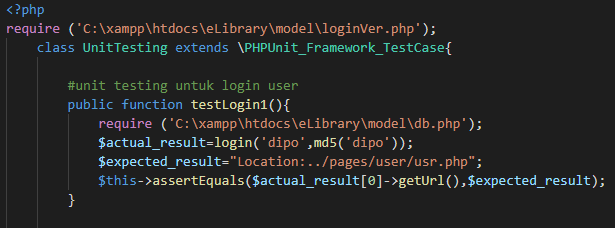
\includegraphics[scale=1.00]{../DokumenSkripsi/gambar/implementasi1}
			\centering
			\caption{\textit Contoh {unit testing} yang dibuat secara manual}
		\end{figure}
Pada gambar 12 dapat terlihat \textit{unit testing} yang dibuat secara manual, \textit{unit testing} tersebut lah yang akan digunakan sebagai rancangan untuk membuat perangkat lunak \textit{auto-generate unit testing} yang dimana nantinya, perangkat lunak akan menghasilkan file berformat php yang memiliki kode-kode seperti pada gambar 12. \textit{Unit testing} akan dilakukan berdasarkan fitur-fitur yang ada pada \textit{website} e-library, yaitu ada 5 fitur, \textit{login, signup, addAdmin, addBook, }dan \textit{updateUser}, dimana output perangkat lunak ini akan menghasilkan \textit{unit testing} dari masing-masing fitur yang ada.

\begin{figure}[h!]
			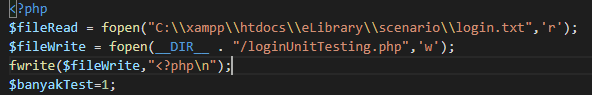
\includegraphics[scale=1.00]{../DokumenSkripsi/gambar/implementasi2}
			\centering
			\caption{\textit Contoh {unit testing} yang dibuat secara manual}
		\end{figure}

Langkah pertama yang dilakukan pada perangkat lunak ini yaitu membaca file skenario Gherkin yang sudah diberikan oleh \textit{stakeholder} kepada \textit{developer}. Seperti dapat dilihat pada gambar 13, perangkat lunak membaca file menggunakan metode fopen dari file berformat txt dengan nama \textbf{login}, dimana skenario tersebut merupakan skenario Gherkin untuk fitur login, dan ditampung pada variabel \texttt{\$fileRead}. Tahap selanjutnya yaitu, menyiapkan sebuah variabel dijadikan hasil/\textit{output} dari perangkat lunak ini, dimana hasil akhirnya dapat dilihat pada gambar 13 yaitu file berformat php dengan nama \textbf{loginUnitTesting}, variabel tersebut yaitu \texttt{\$fileWrite}.


		\item \textbf{Menulis dokumen skripsi.}\\ 
		{\bf Status :} Ada sejak rencana kerja skripsi.\\
		{\bf Hasil :} Menulis dokumen skripsi sudah dilakukan untuk Bab 1 dan Bab 2.

	\end{enumerate}

\section{Pencapaian Rencana Kerja}
Langkah-langkah kerja yang berhasil diselesaikan dalam Skripsi 1 ini adalah sebagai berikut:
\begin{enumerate}
\item Studi literatur mengenai pengujian perangkat lunak, \textit{unit testing}, dan \textit{behaviour specification.}
\item Melakukan Eksplorasi perangkat lunak.
\item Menganalisis kebutuhan perangkat lunak.
\item Membuat rancangan desain antarmuka perangkat lunak.
\item Mempelajari framework PHPUnit.
\item Melakukan analisis masalah.
\item Merancang perangkat lunak tahap awal.
\item Memodifikasi website agar bisa dilakukan \textit{Unit Testing}.
\item Melakukan implementasi perangkat lunak.
\item Melaporkan hasil penelitian dalam bentuk dokumen skripsi

\end{enumerate}



\section{Kendala yang Dihadapi}
%TULISKAN BAGIAN INI JIKA DOKUMEN ANDA TIPE A ATAU C
Kendala - kendala yang dihadapi selama mengerjakan skripsi :
\begin{itemize}
	\item Mengatur waktu antara kuliah, tugas, dan skripsi.
	\item Sakit.
	\item Pandemi membuat kondisi perkuliahan menjadi sulit dan juga membuat resah.
\end{itemize}

\vspace{1cm}
\centering Bandung, \tanggal\\
\vspace{2cm} \nama \\ 
\vspace{1cm}

Menyetujui, \\
\ifdefstring{\jumpemb}{2}{
\vspace{1.5cm}
\begin{centering} Menyetujui,\\ \end{centering} \vspace{0.75cm}
\begin{minipage}[b]{0.45\linewidth}
% \centering Bandung, \makebox[0.5cm]{\hrulefill}/\makebox[0.5cm]{\hrulefill}/2013 \\
\vspace{2cm} Nama: \pembA \\ Pembimbing Utama
\end{minipage} \hspace{0.5cm}
\begin{minipage}[b]{0.45\linewidth}
% \centering Bandung, \makebox[0.5cm]{\hrulefill}/\makebox[0.5cm]{\hrulefill}/2013\\
\vspace{2cm} Nama: \pembB \\ Pembimbing Pendamping
\end{minipage}
\vspace{0.5cm}
}{
% \centering Bandung, \makebox[0.5cm]{\hrulefill}/\makebox[0.5cm]{\hrulefill}/2013\\
\vspace{2cm} Nama: \pembA \\ Pembimbing Tunggal
}
\end{document}

